% Diseño experimental: particiones de CCT (CCT-20 y dataset completo), modelos A y B, y análisis. Standalone, insertar el PDF.
\documentclass[tikz,border=2pt]{standalone}
\usepackage[T1]{fontenc}
\usepackage{mathptmx}
\usetikzlibrary{positioning,arrows.meta,calc,fit,backgrounds}
\definecolor{azul}{HTML}{1F3B5C}\definecolor{gris}{HTML}{8A8F98}
\definecolor{oxido}{HTML}{B5523B}\definecolor{ocre}{HTML}{C98B2B}\definecolor{verde}{HTML}{5B7F4A}
\begin{document}
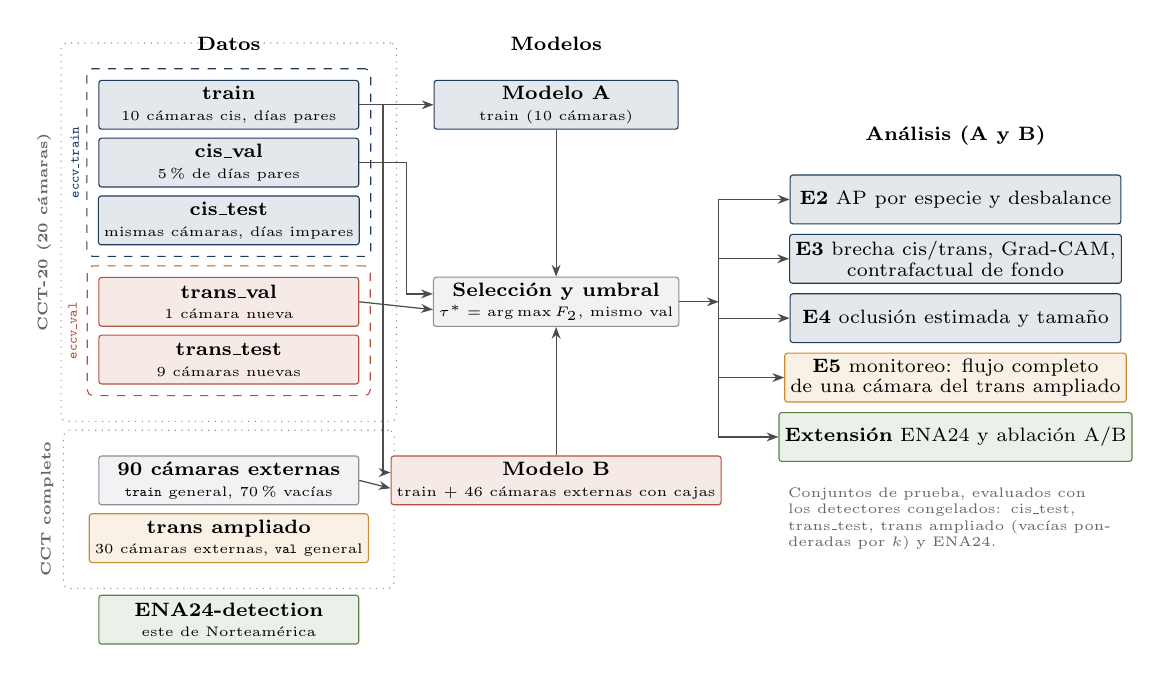
\begin{tikzpicture}[font=\scriptsize, >={Stealth[length=1.5mm]},
  caja/.style={draw=#1, fill=#1!12, rounded corners=1pt, align=center, inner sep=2pt, minimum height=6.2mm, minimum width=33mm, line width=.4pt},
  caja/.default=azul, f/.style={->, draw=black!70, line width=.45pt}, fd/.style={->, draw=gris, dashed, line width=.45pt}]
% ---------------- datos ----------------
\node[caja=azul] (tr) {\textbf{train}\\[-.2mm]{\tiny 10 cámaras cis, días pares}};
\node[caja=azul, below=1mm of tr] (cv) {\textbf{cis\_val}\\[-.2mm]{\tiny 5\,\% de días pares}};
\node[caja=azul, below=1mm of cv] (ct) {\textbf{cis\_test}\\[-.2mm]{\tiny mismas cámaras, días impares}};
\node[caja=oxido, below=4mm of ct] (tv) {\textbf{trans\_val}\\[-.2mm]{\tiny 1 cámara nueva}};
\node[caja=oxido, below=1mm of tv] (tt) {\textbf{trans\_test}\\[-.2mm]{\tiny 9 cámaras nuevas}};
\node[caja=gris, below=9mm of tt] (et) {\textbf{90 cámaras externas}\\[-.2mm]{\tiny \texttt{train} general, 70\,\% vacías}};
\node[caja=ocre, below=1mm of et] (ev) {\textbf{trans ampliado}\\[-.2mm]{\tiny 30 cámaras externas, \texttt{val} general}};
\node[caja=verde, below=4mm of ev] (en) {\textbf{ENA24-detection}\\[-.2mm]{\tiny este de Norteamérica}};
\begin{scope}[on background layer]
\node[draw=azul, dashed, rounded corners=2pt, fit=(tr)(ct), inner sep=1.4mm] (fe1) {};
\node[draw=oxido, dashed, rounded corners=2pt, fit=(tv)(tt), inner sep=1.4mm] (fe2) {};
\node[draw=gris, dotted, rounded corners=2pt, fit=(fe1)(fe2), inner sep=3.2mm] (f20) {};
\node[draw=gris, dotted, rounded corners=2pt, fit=(et)(ev), inner sep=3.2mm] (fext) {};
\end{scope}
\node[font=\tiny, text=azul, rotate=90, anchor=south] at ($(fe1.west)+(.3mm,0)$) {\texttt{eccv\_train}};
\node[font=\tiny, text=oxido, rotate=90, anchor=south] at (fe2.west) {\texttt{eccv\_val}};
\node[font=\tiny\bfseries, text=gris!70!black, rotate=90, anchor=south] at (f20.west) {CCT-20 (20 cámaras)};
\node[font=\tiny\bfseries, text=gris!70!black, rotate=90, anchor=south, align=center] at (fext.west) {CCT completo};
\node[font=\scriptsize\bfseries, above=2.5mm of tr] {Datos};
% ---------------- modelos ----------------
\node[caja=azul, minimum width=31mm] (mA) at ($(tr.east)+(25mm,0)$) {\textbf{Modelo A}\\[-.2mm]{\tiny train (10 cámaras)}};
\node[caja=oxido, minimum width=31mm] (mB) at (mA |- et) {\textbf{Modelo B}\\[-.2mm]{\tiny train + 46 cámaras externas con cajas}};
\node[caja=gris, minimum width=31mm] (sel) at (mA |- tv) {\textbf{Selección y umbral}\\[-.2mm]{\tiny $\tau^\ast=\arg\max F_2$, mismo val}};
\draw[f] (tr.east) -- (mA.west);
\draw[f] (tr.east) -- ++(3mm,0) |- ($(mB.west)+(0,1mm)$);
\draw[f] (et.east) -- ($(mB.west)+(0,-1mm)$);
\draw[f] (cv.east) -- ++(6mm,0) |- ($(sel.west)+(0,1mm)$);
\draw[f] (tv.east) -- ($(sel.west)+(0,-1mm)$);
\draw[f] (mA) -- (sel); \draw[f] (mB) -- (sel);
\node[font=\scriptsize\bfseries, above=2.5mm of mA] {Modelos};
% ---------------- análisis ----------------
\node[caja=azul, minimum width=42mm, anchor=west] (e2) at ($(sel.east)+(14mm,13mm)$) {\textbf{E2} AP por especie y desbalance};
\node[caja=azul, minimum width=42mm, below=1.2mm of e2] (e3) {\textbf{E3} brecha cis/trans, Grad-CAM,\\[-.2mm] contrafactual de fondo};
\node[caja=azul, minimum width=42mm, below=1.2mm of e3] (e4) {\textbf{E4} oclusión estimada y tamaño};
\node[caja=ocre, minimum width=42mm, below=1.2mm of e4] (e5) {\textbf{E5} monitoreo: flujo completo\\[-.2mm] de una cámara del trans ampliado};
\node[caja=verde, minimum width=42mm, below=1.2mm of e5] (ex) {\textbf{Extensión} ENA24 y ablación A/B};
\node[font=\scriptsize\bfseries, above=2.5mm of e2] {Análisis (A y B)};
\draw[f] (sel.east) -- ++(5mm,0) coordinate (dd);
\foreach \n in {e2,e3,e4,e5,ex} \draw[f] (dd) |- (\n.west);
\node[font=\tiny, text=gris!70!black, align=left, anchor=north west, text width=42mm] at ($(ex.south west)+(0,-2mm)$)
  {Conjuntos de prueba, evaluados con los detectores congelados: cis\_test, trans\_test, trans ampliado (vacías ponderadas por $k$) y ENA24.};
\end{tikzpicture}
\end{document}
